\documentclass[12pt]{article}
\usepackage{czech}
\usepackage[utf8]{inputenc}
\usepackage[plainpages=false,pdfpagelabels,unicode]{hyperref}
\usepackage[pdftex]{graphicx}
\usepackage[margin=3cm, includefoot]{geometry}

\begin{document}

\title{Zpráva o praxi v HVM Plasma s. r. o.}
\author{Pavel Ondračka}
\maketitle

\section{O firmě}
HVM Plasma je Česká firma založená v roce 1992 jež se zabývá technologiemi pov\-la\-ko\-vá\-ní metodami PVD\footnote{Physical Vapour Deposition} a PACVD\footnote{Plasma Assisted Chemical Vapour Deposition}. Jedná se konkrétně o vývoj, konstrukce a výrobu vakuových zařízení, zakázkové povlakování, vývoj nových technologií povlakování a měření vlastností tenkých vrstev. Firma má v současné době asi 75 zaměstnanců, centrála sídlí v Praze, s výrobními středisky taktéž v Praze a v Brně. Moje odborná praxe probíhala právě ve výrobním středisku v Brně Modřicích.

\subsection{Technologie depozice tenkých vrstev}
Pro výrobu povlaků a tenkých vrstev se ve firmě HVM Plasma používají reaktory od firmy Hauzer Techno Coating. V Brněnském povlakovacím středisku je celkem pět reaktorů: modely HTC1200, HTC1500 a HTC625. Technologie depozice je jednak magnetronové naprašování, a také PACVD  využívající stejnosměrné pulzní napětí. Těmito postupy je vyráběno široké spektrum vrstev, například povlaky: TiN, TiCN, Cr, CrN, Me-C:H a DLC\footnote{Diamond Like Carbon}, případně jejich kombinace. Při depozicích je potřeba vysokého vakua, k tomu slouží čerpací systém složení z olejových a turbomolekulárních vývěv. Čistoty dílů před depozicí se dosahuje jednak díky praní ve speciální ultrazvukové vícestupňové myčce na vodní bázi, jedna plazmovým čištěním před zahájením depozice.  

\begin{figure}[htbp]
\centering
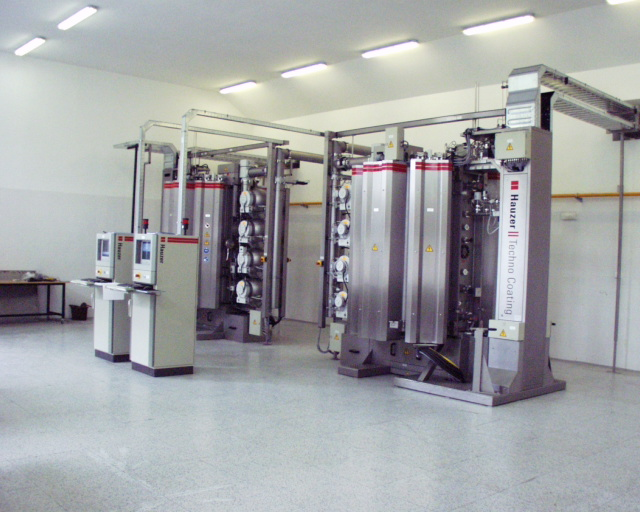
\includegraphics[width=280px]{htc1500.jpg}
\caption{Hauser Techno Coatings HTC1500}
\label{htc1500}
\end{figure}

\begin{figure}[htbp]
\centering
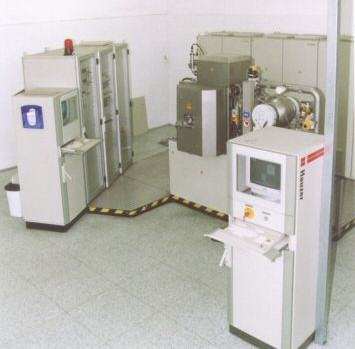
\includegraphics[width=280px]{htc625.jpg}
\caption{Hauser Techno Coatings HTC1500}
\label{htc625}
\end{figure}

\subsection{Kontrola kvality}
Jelikož mají zákazníci vysoké nároky na kvalitu výroby a povlakování, je potřeba provádět kontroly dílů jednak před povlakováním a také po povlakování. Požadované parametry závisejí na konkrétním zákazníkovi a procesu, ovšem některé významné parametry se měří pro většinu vrstev. Jedná se konkrétně o adhezi, tloušťku vrstvy, drsnost a mikrotvrdost. Dále se kontrolují geometrické parametry výrobku, například pro písty je to kruhovitost, válcovitost, přímost atd. Jelikož jsem většinu své praxe strávil právě v laboratoři kontroly kvality, následuje krátký souhrn používaných metod.


\subsubsection{Tloušťka vrstvy}
Tloušťka vrstev je v HVM měřena pomocí tzv. kalotestu. Pomocí koule o definovaném průměru potřené diamantovou pastou se do vrstvy vybrousí kruhový vrchlík, tzv. kalota. Ta je poté zkoumána na mikroskopu a jsou odečteny průměry kružnic ohraničujících vrstvu a substrát, ze kterých je následně vypočítána tloušťka vrstvy. Výhoda toho postupu je, že se dá dobře použít i pro multivrstvy, a zjistit tloušťku jednotlivých vrstev (někdy je potřeba použít kyselinu na zvýšení kontrastu). Nevýhodou kalotestu je požadavek poměrně hladkého povrchu. 

\begin{figure}[!ht]

\begin{minipage}[b]{0.5\linewidth}
\centering
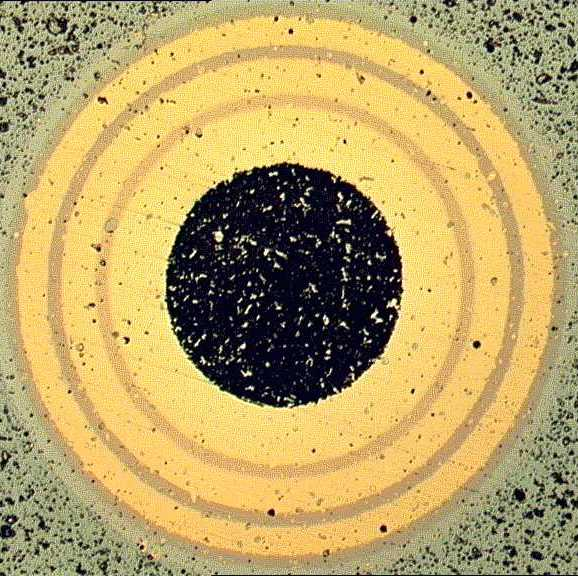
\includegraphics[height=150px]{calo_d.jpg}
\caption{Kalota na multivrstvě}
\label{kalota}
\end{minipage}
\begin{minipage}[b]{0.5\linewidth}
\centering
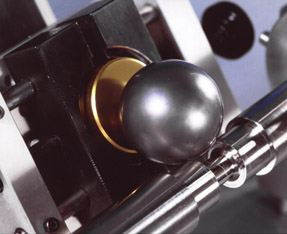
\includegraphics[height=150px]{calo_e.jpg}
\caption{Kalotest}
\label{kalotest}
\end{minipage}

\hspace{1.5cm}

\begin{minipage}[b]{0.5\linewidth}
\centering
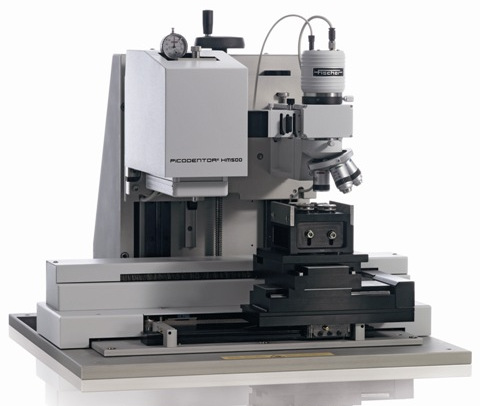
\includegraphics[height=140px]{picodentor.jpg}
\caption{Mikrotvrdoměr HM1500}
\label{mikrotvrdomer}
\end{minipage}
\begin{minipage}[b]{0.5\linewidth}
\centering
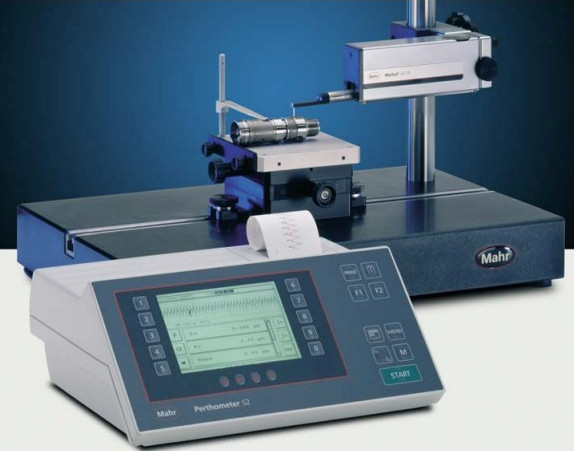
\includegraphics[height=140px]{drsnomer.jpg}
\caption{Drsnoměr Perthometer S2}
\label{drsnomer}
\end{minipage}

\end{figure}

\subsubsection{Mikrotvrdost}
Je určována zejména pro tenké vrstvy, definice je stejná jako u klasické tvrdosti, ale hlavní rozdíl spočívá ve volbě velikosti maximální zátěže. V tomto případě je maximální zátěž v řádu desítek mN. Důvodem použití tak nízkých zátěžných sil spočívá v nutnosti měření tvrdosti samotné vrstvy bez vlivu materiálu na kterém je vrstva nanesena. Hlavní výhodou těchto typů přístrojů je měření tvrdosti v průběhu zatěžování i během odtěžování. Výsledkem měření je pak nejen výsledné číslo odpovídající tvrdosti materiálu, ale i tvar zatěžovací a odtěžovací křivky. Na ní je možné rozpoznat nejen nehomogenity, vměstky v různých hloubkách apod., ale mezi hlavní výhody patří rozpoznání podílu elastické a plastické deformace.  

\subsubsection{Drsnost}
Je souhrn nerovností povrchu s relativně malou vzdáleností, které nevyhnutelně vznikají při výrobě nebo jejím vlivem. V případě nanášení PVD vrstev je drsnost způsobená jak vlastním opracováním nástroje, tak i odprašovaným materiálem, který je deponován na nástroj. Při měření drsnosti se nepočítají vady povrchu, tj. náhodné nepravidelné nerovnosti, které se vyskytují jen ojediněle (rysky, trhlinky, důlky apod.) a které vznikají vadami materiálu, poškozením aj.

\subsubsection{Adheze}
Jedná se vyhodnocování přilnavosti vrstvy k povlakovanému nástroji. V HVM jsou využívány dvě metody pro měření adheze povlaků k substrátu.

Scratch test -- při vyhodnocování se využívá principu postupně se zvyšující zátěžné síly na diamantový Rockwellův hrot při současném posouvání špičky hrotu po měřené vrstvě. S ohledem na běžné velikosti přilnavosti se prakticky používá zátěžná síla v rozsahu 20 - 120N. Při měření vrstvy je detekována akustická emise, která se mění při odtržení vrstvy což koresponduje s určitou hodnotou zátěže. Tato kritická hodnota při které dochází k odtržení vrstvy se označuje jako adheze vrstvy. Navíc je možné provést závěrečnou kontrolu pomocí optického mikroskopu. Pomocí mikroskopu se určí na vzniklé dráze místo, kde došlo k odtržení vrstvy a je odečtena přesná hodnota kritické zátěže.

Rockwell -- provozní metoda měření adheze, která se měří pomocí Rockwellova tvrdoměru. Opticky se hodnotí vtisk Rockwellova hrotu na pomocném vzorku, respektive odlupování vrstvy v jeho okolí. K hodnocení slouží empirická stupnice HF0 až HF8, kdy vyhovující adheze je HF0 až HF3.

\section{Průběh praxe}
V prvních dnech jsem byl seznámen s činností firmy, s používanými technologiemi, pracovními postupy, výrobou a činností laboratoře na kontrolu kvality. Zbytek času jsem strávil v laboratoři měřením vyrobených dílů především pak adheze, drsnosti, tloušťky a geometrických parametrů. Jednalo se o hlavně o povlaky Cr2N a wolfram-chrom-DLC na výrobky pro automobilový průmysl. Ke konci praxe jsem již byl schopen samostatně a úspěšně vykonávat většinu činností v laboratoři. Trvání praxe bylo od 1.8.2012 do 31.8.2012, celkově se jednalo o 

\section{Závěr}
Praxe v HMV pro mě byla velmi užitečná. Jednak jako seznámení s dalšími depozičními postupy, které jsem dříve neznal (například použití pulzního DC napětí při depozicích versus použití 12,56\,MHz kapacitně vázaného výboje používaného v reaktorech na ústavu fyzikální elektroniky), což pro mě bude přínosné při dalším studiu fyziky plazmatu. Další velkou zkušeností bylo seznámení se s prostředím průmys\-lo\-vé výroby. Cennou zkušeností byla i praxe v laboratoři a práce s měřícími přístroji.

\end{document}

%FIXME:d
